\documentclass[unknownkeysallowed]{beamer}
\usepackage[french,english]{babel}
\usepackage{../sty/beamer_js}
\usepackage{../sty/shortcuts_js}
\usepackage{listings}


\addbibresource{../biblio/references_all.bib}

\begin{document}


%%%%%%%%%%%%%%%%%%%%%%%%%%%%%%%%%%%%%%%%%%%%%%%%%%%%%%%%%%%%%%%%%%%%%%%%%%%%%%%
%%%%%%%%%%%%%%%%%%%%%%             Headers               %%%%%%%%%%%%%%%%%%%%%%
%%%%%%%%%%%%%%%%%%%%%%%%%%%%%%%%%%%%%%%%%%%%%%%%%%%%%%%%%%%%%%%%%%%%%%%%%%%%%%%



%%%%%%%%%%%%%%%%%%%%%%%%%%%%%%%%%%%%%%%%%%%%%%%%%%%%%%%%%%%%%%%%%%%%%%%%%%%%%%%
\begin{frame}
\bigskip
\bigskip
\begin{center}{
\LARGE\color{marron}
\textbf{HMM307: Modèles linéaires avancés}
\textbf{ }\\
\vspace{0.5cm}
}

\color{marron}
\textbf{Maximum de vraisemblance vs. Maximum de vraisemblance restreint}
\end{center}

\vspace{0.5cm}

\begin{center}
\textbf{Mégane Diéval} \\
\vspace{0.1cm}
\url{https://github.com/MegDie/ML_VS_REML}\\
\vspace{0.5cm}
Université de Montpellier \\
\end{center}

\centering
\includegraphics[width=0.13\textwidth]{Logo}

\end{frame}
%%%%%%%%%%%%%%%%%%%%%%%%%%%%%%%%%%%%%%%%%%%%%%%%%%%%%%%%%%%%%%%%%%%%%%%%%%%%%%%



%%%%%%%%%%%%%%%%%%%%%%%%%%%%%%%%%%%%%%%%%%%%%%%%%%%%%%%%%%%%%%%%%%%%%%%%%%%%%%%
%%%%%%%%%%%%%%%%%%%%%%%%       PLAN      %%%%%%%%%%%%%%%%%%%%%%%%%%%%%%%%%%%%%%
%%%%%%%%%%%%%%%%%%%%%%%%%%%%%%%%%%%%%%%%%%%%%%%%%%%%%%%%%%%%%%%%%%%%%%%%%%%%%%%



%%%%%%%%%%%%%%%%%%%%%%%%%%%%%%%%%%%%%%%%%%%%%%%%%%%%%%%%%%%%%%%%%%%%%%%%%%%%%%%
\begin{frame}{Sommaire}
\tableofcontents[hideallsubsections]
\end{frame}
%%%%%%%%%%%%%%%%%%%%%%%%%%%%%%%%%%%%%%%%%%%%%%%%%%%%%%%%%%%%%%%%%%%%%%%%%%%%%%%



%%%%%%%%%%%%%%%%%%%%%%%%%%%%%%%%%%%%%%%%%%%%%%%%%%%%%%%%%%%%%%%%%%%%%%%%%%%%%%%
\AtBeginSection[]
{
\begin{frame}<beamer>{Sommaire}
\tableofcontents[currentsubsection,
    hideothersubsections,
    sectionstyle=show/shaded,
]
\end{frame}
}
%%%%%%%%%%%%%%%%%%%%%%%%%%%%%%%%%%%%%%%%%%%%%%%%%%%%%%%%%%%%%%%%%%%%%%%%%%%%%%%




%%%%%%%%%%%%%%%%%%%%%%%%%%%%%%%%%%%%%%%%%%%%%%%%%%%%%%%%%%%%%%%%%%%%%%%%%%%%%%%
%%%%%%%%%%%%%%%%%%%%%%%%%%%%%%%%%%%%%%%%%%%%%%%%%%%%%%%%%%%%%%%%%%%%%%%%%%%%%%%
\section{Les estimateurs du maximum de vraisemblance (ML)}
\label{sec:introdcution}
%%%%%%%%%%%%%%%%%%%%%%%%%%%%%%%%%%%%%%%%%%%%%%%%%%%%%%%%%%%%%%%%%%%%%%%%%%%%%%
%%%%%%%%%%%%%%%%%%%%%%%%%%%%%%%%%%%%%%%%%%%%%%%%%%%%%%%%%%%%%%%%%%%%%%%%%%%%%%%

%%%%%%%%%%%%%%%%%%%%%%%%%%%%%%%%%%%%%%%%%%%%%%%%%%%%%%%%%%%%%%%%%%%%%%%%%%%%%%%
\subsection{Présentation du problème}
\label{sub:un_premier_exemple}
%%%%%%%%%%%%%%%%%%%%%%%%%%%%%%%%%%%%%%%%%%%%%%%%%%%%%%%%%%%%%%%%%%%%%%%%%%%%%%%

\begin{frame}{La problématique des estimateurs biaisés}

\begin{figure}
    \centering
    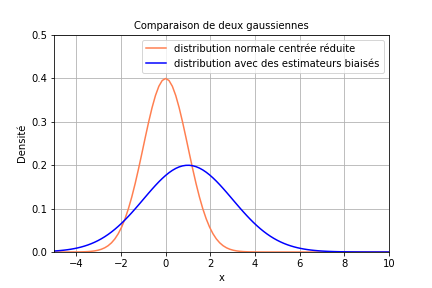
\includegraphics[width=0.9\textwidth]{tex/draft-beamer/prebuiltimages/normal_distribution.png}
    \caption{La courbe bleue est une estimation de la courbe orange par des paramètres biaisés}
    \label{fig:my_label}
\end{figure}
    
\end{frame}
%%%%%%%%%%%%%%%%%%%%%%%%%%%%%%%%%%%%%%%%%%%%%%%%%%%%%%%%%%%%%%%%%%%%%%%%%%%%%%%

%%%%%%%%%%%%%%%%%%%%%%%%%%%%%%%%%%%%%%%%%%%%%%%%%%%%%%%%%%%%%%%%%%%%%%%%%%%%%%%
\subsection{Un estimateur de la variance biaisé}
\label{sub:deuxiem_exmple}
%%%%%%%%%%%%%%%%%%%%%%%%%%%%%%%%%%%%%%%%%%%%%%%%%%%%%%%%%%%%%%%%%%%%%%%%%%%%%%%

%%%%%%%%%%%%%%%%%%%%%%%%%%%%%%%%%%%%%%%%%%%%%%%%%%%%%%%%%%%%%%%%%%%%%%%%%%%%%%%
\begin{frame}{Rappels sur les modèles linéaires mixtes}

\mytheorem{Le modèle linéaire mixte}{


    $$Y = X\beta + K\alpha + \epsilon$$
    $$avec \ Y \in \mathbb{R}^n, \ X \in \mathbb{R}^{n \times q}, \ K \in \mathbb{R}^{n \times q}, \ \beta \in \mathbb{R}^q, \ \alpha \in \mathbb{R}^q, \ \epsilon \in \mathbb{R}^n$$
    $$\epsilon \sim \mathcal{N}(0,\sigma^2_\epsilon Id_n), \   \alpha_j \sim \mathcal{N}(0,\sigma^2_j Id_{q_j}) , \ Y \sim \mathcal{N}(X\beta, Var (Y)) $$
    $$Var(Y) = \Sigma_y =  Var(\epsilon) + Var (K\alpha)$$


}

\vspace{0.25cm}

\begin{itemize}
	\item $X$ est l'effet fixe du modèle et ne comporte pas d'erreur
	\item $K$ est l'effet aléatoire du modèle
	\item $\epsilon$ est le bruit du modèle 
\end{itemize}



    
\end{frame}

%%%%%%%%%%%%%%%%%%%%%%%%%%%%%%%%%%%%%%%%%%%%%%%%%%%%%%%%%%%%%%%%%%%%%%%%%%%%%%%
\begin{frame}{Les estimateurs du maximum de vraisemblance}

\vspace{0.4cm}

\mytheorem{Estimateurs \rm{ML} de $\beta$ et de la variance}
{

$$\hat{\beta} = (X^t X)^{-1} \ X^{t} \ Y$$ 
$$\hat{\Sigma_y} = \frac{1}{n} \ (Y-X\hat{\beta})^t \ (Y-X\hat{\beta})$$

}


\vspace{0.25cm}

L'estimation de la variance \mybold{dépend d'un estimateur qui peut comporter une erreur}.

\vspace{0.25cm}

$\mathbb{E}[\hat{\Sigma_y}] = \frac{n-q}{n} \ \Sigma_y$ 

\vspace{0.25cm}

\begin{itemize}
	\item Sous-estimation de la vraie variance
	\item Erreur d'autant plus grande que $q \approx n$
\end{itemize}


\end{frame}
%%%%%%%%%%%%%%%%%%%%%%%%%%%%%%%%%%%%%%%%%%%%%%%%%%%%%%%%%%%%%%%%%%%%%%%%%%%%%%%


%%%%%%%%%%%%%%%%%%%%%%%%%%%%%%%%%%%%%%%%%%%%%%%%%%%%%%%%%%%%%%%%%%%%%%%%%%%%%%%
%%%%%%%%%%%%%%%%%%%%%%%%%%%%%%%%%%%%%%%%%%%%%%%%%%%%%%%%%%%%%%%%%%%%%%%%%%%%%%%
\section{L'estimateur REML, une solution}
\label{sec:conclusion}
%%%%%%%%%%%%%%%%%%%%%%%%%%%%%%%%%%%%%%%%%%%%%%%%%%%%%%%%%%%%%%%%%%%%%%%%%%%%%%%
%%%%%%%%%%%%%%%%%%%%%%%%%%%%%%%%%%%%%%%%%%%%%%%%%%%%%%%%%%%%%%%%%%%%%%%%%%%%%%%


%%%%%%%%%%%%%%%%%%%%%%%%%%%%%%%%%%%%%%%%%%%%%%%%%%%%%%%%%%%%%%%%%%%%%%%%%%%%%%%
\begin{frame}{L'estimateur REML, une solution}

\mybold{Stratégie :} Exprimer la log-vraisemblance en se passant de l'information sur la moyenne.

\vspace{4mm}

\begin{itemize}
\visible<2->{\item 1) Intégrer par rapport à $\beta$ pour se passer de l'information estimée: 

\[L(\beta, \sigma_j^2, \sigma_{\epsilon}^2) = \frac{1}{\sqrt{2\pi |\Sigma_y|}}e^{-\frac{\trans{(Y-X\beta)}\Sigma_y^{-1}(Y-X\beta)}{2}}\]

}

\only<3->{\item 2) Utiliser cette expression pour calculer la log-vraisemblance:

\vspace{2mm}

$$-\frac{1}{2}log(2\pi)-\frac{1}{2}log(|\Sigma_y|)+log\left[\int e^{-\frac{\trans{(Y-X\beta)}\Sigma_y^{-1}(Y-X\beta)}{2}} d\beta\right]$$



}

\end{itemize}

\end{frame}
%%%%%%%%%%%%%%%%%%%%%%%%%%%%%%%%%%%%%%%%%%%%%%%%%%%%%%%%%%%%%%%%%%%%%%%%%%%%%%%

%%%%%%%%%%%%%%%%%%%%%%%%%%%%%%%%%%%%%%%%%%%%%%%%%%%%%%%%%%%%%%%%%%%%%%%%%%%%%%%
\begin{frame}{L'estimateur REML, une solution}

\mybold{Stratégie :} Exprimer la log-vraisemblance en se passant de l'information sur la moyenne.

\vspace{4mm}

\begin{itemize}
\visible<1->{\item 3) Réaliser un développement de Taylor sur l'exposant de l'exponentielle:

$$f(\beta)=\frac{\trans{(Y-X\beta)}\Sigma_y^{-1}(Y-X\beta)}{2}$$ 

$$f(\beta)\approx f(\hat{\beta})+(1/2)(\beta-\hat{\beta})^2f''(\hat{\beta})$$
}

\only<2->{\item 4)
 Identifier le biais après avoir calculé la log-vraisemblance de cette façon: 

$$- \frac{1}{2}\log{\left(\lvert\Sigma_y\rvert\right)}-\frac{1}{2}\displaystyle \left(Y-X\hat{\beta}\right)^T\Sigma_y^{-1}\left(Y-X\hat{\beta}\right)-\frac{1}{2}\log\left(|X^T\Sigma_y^{-1}X|\right)$$

}

\end{itemize}
	

\end{frame}
%%%%%%%%%%%%%%%%%%%%%%%%%%%%%%%%%%%%%%%%%%%%%%%%%%%%%%%%%%%%%%%%%%%%%%%%%%%%%%%


%%%%%%%%%%%%%%%%%%%%%%%%%%%%%%%%%%%%%%%%%%%%%%%%%%%%%%%%%%%%%%%%%%%%%%%%%%%%%%%
%%%%%%%%%%%%%%%%%%%%%%%%%%%%%%%%%%%%%%%%%%%%%%%%%%%%%%%%%%%%%%%%%%%%%%%%%%%%%%%
\section{Un exemple concret}
\label{sec:conclusion}
%%%%%%%%%%%%%%%%%%%%%%%%%%%%%%%%%%%%%%%%%%%%%%%%%%%%%%%%%%%%%%%%%%%%%%%%%%%%%%%
%%%%%%%%%%%%%%%%%%%%%%%%%%%%%%%%%%%%%%%%%%%%%%%%%%%%%%%%%%%%%%%%%%%%%%%%%%%%%%%


%%%%%%%%%%%%%%%%%%%%%%%%%%%%%%%%%%%%%%%%%%%%%%%%%%%%%%%%%%%%%%%%%%%%%%%%%%%%%%%
\subsection{Présentation du jeu de données}
\label{sub:rapidement}
%%%%%%%%%%%%%%%%%%%%%%%%%%%%%%%%%%%%%%%%%%%%%%%%%%%%%%%%%%%%%%%%%%%%%%%%%%%%%%%



%%%%%%%%%%%%%%%%%%%%%%%%%%%%%%%%%%%%%%%%%%%%%%%%%%%%%%%%%%%%%%%%%%%%%%%%%%%%%%%
\begin{frame}{Présentation du jeu de données}

	 \begin{table}
        \centering
        \begin{tabular}{| c | c | c|}
        \hline
        \begin{bf} Ind \end{bf} &
        \begin{bf} Resp \end{bf} &
        \begin{bf} Treat \end{bf} \\
        \hline
        1 &  10 & 0\\
        1 & 25 & 1 \\
        2 & 3 & 0 \\
        2 &  6 & 1\\
        \hline
        \end{tabular}
    \caption{jeu de données}
    \end{table}

\vspace{4mm}

\emph{Treat} : Indicatrice du traitement \newline
\emph{Resp} : Variable d'intérêt \newline
\emph{Ind} : Indicatrice d'individu

\end{frame}
%%%%%%%%%%%%%%%%%%%%%%%%%%%%%%%%%%%%%%%%%%%%%%%%%%%%%%%%%%%%%%%%%%%%%%%%%%%%%%%


%%%%%%%%%%%%%%%%%%%%%%%%%%%%%%%%%%%%%%%%%%%%%%%%%%%%%%%%%%%%%%%%%%%%%%%%%%%%%%%
\begin{frame}{4 données qui conservent les propriétés du modèle linéaire mixte}

\begin{figure}[H]
\centering
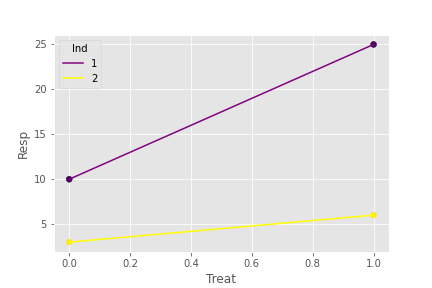
\includegraphics[width = 0.8\textwidth]{tex/draft-beamer/prebuiltimages/points.png}
\caption{Représentation graphique du jeu de données}
\end{figure}

\mybold{Modèle} : $Y_{Resp} = X_{Treat} \ \beta + K_{Ind} \ \alpha + \epsilon$


\end{frame}
%%%%%%%%%%%%%%%%%%%%%%%%%%%%%%%%%%%%%%%%%%%%%%%%%%%%%%%%%%%%%%%%%%%%%%%%%%%%%%%

%%%%%%%%%%%%%%%%%%%%%%%%%%%%%%%%%%%%%%%%%%%%%%%%%%%%%%%%%%%%%%%%%%%%%%%%%%%%%%%
\subsection{Calcul des estimateurs selon les deux méthodes}
\label{sub:rapidement}
%%%%%%%%%%%%%%%%%%%%%%%%%%%%%%%%%%%%%%%%%%%%%%%%%%%%%%%%%%%%%%%%%%%%%%%%%%%%%%%

\begin{frame}{Calcul des estimateurs selon les deux méthodes}

\begin{itemize}
    \item Calcul des estimateurs ML :  $\hat{\beta_1}=6.5$ et $\hat{\beta_2}=15.5$
\end{itemize}

\mybold{Commandes Python}: 

mm\_ml = smf.mixedlm("Resp \~ \ Treat", df, groups = df['Ind']) \newline
result\_ml = mm\_ml.fit(reml=False)

\vspace{3mm}

\begin{itemize}
    \item Calcul des estimateurs REML : $\hat{\beta_1}=6.5$ et $\hat{\beta_2}=15.5$
\end{itemize}

\mybold{Commandes Python}: 

result\_reml = mm\_ml.fit()

\vspace{3mm}

\begin{table}[h!]
    \centering
    \begin{tabular}{| c | c | c | c |}
        \hline
        \begin{bf} Méthode \end{bf} &
        \begin{bf} Log-vraisemblance \end{bf} &
        \begin{bf} $\hat{\sigma_{\epsilon}^}2$ \end{bf} &
        \begin{bf} $\hat{\sigma_j^2}$ \end{bf} \\
        \hline
        REML   & -7.89 & 6.00 & 8.15 \\
        ML  & -13.0 & 4.24 & 5.77 \\
        \hline
    \end{tabular}
\end{table} 

\end{frame}


%%%%%%%%%%%%%%%%%%%%%%%%%%%%%%%%%%%%%%%%%%%%%%%%%%%%%%%%%%%%%%%%%%%%%%%%%%%%%%%%
\begin{frame}{Conclusion}

\begin{itemize}
    \item L'estimateur \rm{REML} résout les problèmes de biais de l'estimateur \rm{ML}.
    \item La log-vraisemblance est supérieure avec \rm{REML} mais les coefficients $\beta$ sont les mêmes.
\end{itemize}

\end{frame}




%%%%%%%%%%%%%%%%%%%%%%%%%%%%%%%%%%%%%%%%%%%%%%%%%%%%%%%%%%%%%%%%%%%%%%%%%%%%%%%
\begin{frame}{Bibliographie}
\printbibliography

\begin{itemize}

    \item Nikolay Oskolkov. Maximum Likelihood (ML) vs. Restricted Maximum Likelihood (REML), 2020
    \item Mégane Diéval. Maximum de vraisemblance vs. Maximum de vraisemblance restreint, 2020
    
    \item Joseph Salmon. HMMA307 - Modèles linéaires avancés, 2020
    
\end{itemize}

\end{frame}
 %%%%%%%%%%%%%%%%%%%%%%%%%%%%%%%%%%%%%%%%%%%%%%%%%%%%%%%%%%%%%%%%%%%%%%%%%%%%%%



\end{document}
